% figure-4-a-domain-for-representing-operators-on-bifinites.tex
%
% Source: Carl A. Gunter and Dana S. Scott, "Semantic Domains".
%   physical page 44 of ScottDomains/papers/Gunter Scott 1990.pdf
%   printed page 43
%   section 7.4, "Representing operators on bifinite domains."
%   caption: "Figure 4: A domain for representing operators on bifinites."
%
% What the figure shows: the first three non-trivial stages of the tower
% I, I^+, I^++, I^+++ that section 7.4 builds towards the fixed point of
% D |-> D^+, where D^+ is the domain of ideals over <M(A), |->.  The paper's
% own prose fixes the element counts:
%
%   "At the first step we take the domain I = {bottom} containing only the
%    single point bottom.  At the second step, I+, there are elements
%    a = (bottom,{bottom}) and b = (bottom,{}) with b |- a.  At the third step
%    there are five elements (a,{a}); (a,{b}); (b,{b}); (b,{}); (a,{}) which
%    form the partially ordered set I++ pictured in Figure 4. ...  The next
%    step I+++ has 20 elements (up to equivalence in the sense just mentioned)
%    and it is also pictured in Figure 4."
%
% Transcribed counts, which agree: I^+ 2, I^++ 5, I^+++ 20 (27 vertices).
% The 5 for I^++ is the count that selects the adopted reading of the section
% 7.4 pre-order over the rival Smyth reading, which yields 1, 2, 5, 21; the
% paper's sentence about identifying (a,{a,b}) with (a,{a}) is precisely the
% identification that takes 21 down to 20 at the next stage.
%
% Open vs filled: the paper's own explanation, same paragraph — "each stage of
% the construction is embedded in the next one by the map x |-> (x,{x}).  The
% closed circles in the figure are intended to give a hint of how this
% embedding looks."  So the filled vertices of each stage carry the image of
% the previous stage: 1 filled in I^+, 2 in I^++, 5 in I^+++.  The induced
% order on the 5 filled vertices of I^+++ is a 4-chain with one extra atom over
% the bottom, i.e. a copy of I^++ — checked against the transcribed edges.
%
% Provenance of the geometry, which is not the usual crop-and-trace:
%
%   Vertices.  Measured exactly, from the page content stream.  `mutool draw
%   -F trace` on physical page 44 reports the 27 circles as glyphs 14 (open)
%   and 15 (filled) of Type 3 font T14, with their PDF-point positions.  Every
%   coordinate below is (trace point - (119.76, 251.75)) / 40, so the drawing
%   is the paper's own placement to the point, at 1 cm per 40 pt.
%
%   Edges.  NOT available in that file.  Page 44's raster layer is a 30-byte
%   empty JBIG2 stub (`pdfimages -list`), and the trace shows only text
%   operators and no path operators, so the Paper Capture rebuild that produced
%   `Gunter Scott 1990.pdf` kept the circle glyphs and dropped every connecting
%   line: the figure renders as 27 unconnected dots in poppler and in mupdf
%   alike.  The edges here were recovered from the same figure in the earlier
%   tech report — Figure 1.4, physical page 54 of
%   "Gunter Mosses Scott 1989 Semantic Domains and Denotational Semantics
%   MS-CIS-89-16.pdf", a genuine scan whose lines survive — by measuring all 27
%   circle centres there (scripts/a3-find-circles.py) and testing every vertex
%   pair for ink along the whole segment (scripts/a3-find-edges.py).
%
%   The two drawings share a vertex set but not every position: mapped through
%   an affine fit (scripts/a3-map-vertices.py) the three columns agree to under
%   1 pt, while the 1990 version raised the right-hand arm (R5, R6) and the
%   extra I^++ vertex by one 36 pt step and moved several satellites.  The 1990
%   positions are used here, since that is the paper being transcribed; the
%   1989 scan supplies adjacency only.  The 1990 grid corroborates the
%   assignment: C1, R4, R5, R6 come out exactly collinear (slope 2), as do
%   L6, C5, R2 and L5, C3, R1 (slope -1), which is why the segment test reports
%   those long pairs as covered "via" the middle vertex rather than as edges.
%
% Vertex naming used below: C1..C8 the main column of I^+++ bottom to top,
% L1..L6 its left satellites, R1..R6 its right satellites, B1..B5 the elements
% of I^++, A1..A2 those of I^+.

\documentclass[border=6pt]{standalone}
\usepackage{tikz}
\begin{document}
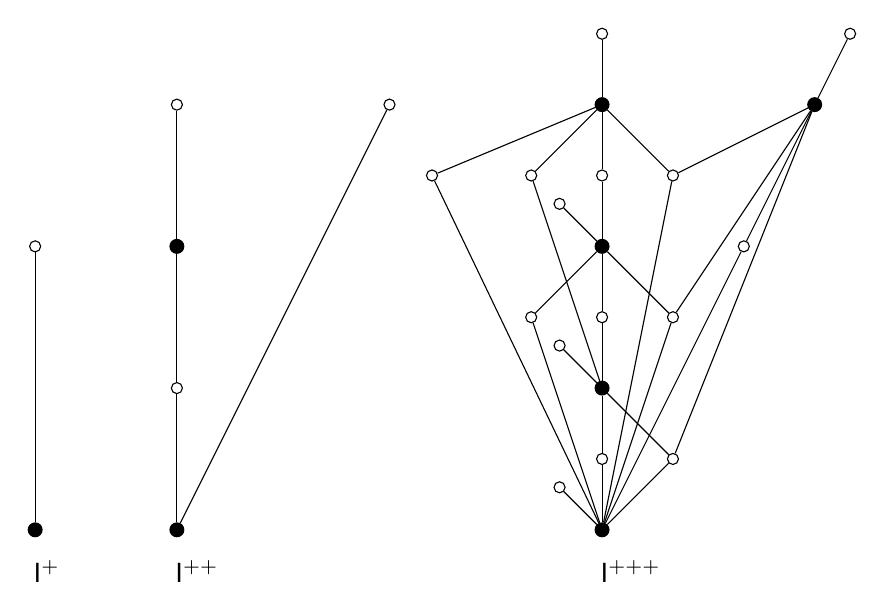
\begin{tikzpicture}[
  x=1cm, y=1cm,
  every node/.style={inner sep=1pt},
  open/.style={circle, draw, fill=white, minimum size=4pt, inner sep=0pt},
  solid/.style={circle, draw, fill=black, minimum size=5pt, inner sep=0pt},
  edge/.style={draw, line width=0.4pt}]

  % ---- vertices -----------------------------------------------------------
  % I^+ : 2 elements, 1 filled
  \node[solid] (A1) at (0,0)       {};
  \node[open]  (A2) at (0,3.6)     {};

  % I^++ : 5 elements, 2 filled
  \node[solid] (B1) at (1.8,0)     {};
  \node[open]  (B2) at (1.8,1.8)   {};
  \node[solid] (B3) at (1.8,3.6)   {};
  \node[open]  (B4) at (1.8,5.4)   {};
  \node[open]  (B5) at (4.5,5.4)   {};

  % I^+++ : 20 elements, 5 filled.  Main column, bottom to top.
  \node[solid] (C1) at (7.2,0)     {};
  \node[open]  (C2) at (7.2,0.9)   {};
  \node[solid] (C3) at (7.2,1.8)   {};
  \node[open]  (C4) at (7.2,2.7)   {};
  \node[solid] (C5) at (7.2,3.6)   {};
  \node[open]  (C6) at (7.2,4.5)   {};
  \node[solid] (C7) at (7.2,5.4)   {};
  \node[open]  (C8) at (7.2,6.3)   {};
  % left satellites
  \node[open]  (L1) at (5.04,4.5)  {};
  \node[open]  (L2) at (6.3,2.7)   {};
  \node[open]  (L3) at (6.3,4.5)   {};
  \node[open]  (L4) at (6.66,0.54) {};
  \node[open]  (L5) at (6.66,2.34) {};
  \node[open]  (L6) at (6.66,4.14) {};
  % right satellites
  \node[open]  (R1) at (8.1,0.9)   {};
  \node[open]  (R2) at (8.1,2.7)   {};
  \node[open]  (R3) at (8.1,4.5)   {};
  \node[open]  (R4) at (9.0,3.6)   {};
  \node[solid] (R5) at (9.9,5.4)   {};
  \node[open]  (R6) at (10.35,6.3) {};

  % ---- edges --------------------------------------------------------------
  % I^+ : 1 edge
  \draw[edge] (A1) -- (A2);

  % I^++ : 4 edges
  \draw[edge] (B1) -- (B2);
  \draw[edge] (B2) -- (B3);
  \draw[edge] (B3) -- (B4);
  \draw[edge] (B1) -- (B5);

  % I^+++ : 28 edges.  Main chain.
  \draw[edge] (C1) -- (C2);
  \draw[edge] (C2) -- (C3);
  \draw[edge] (C3) -- (C4);
  \draw[edge] (C4) -- (C5);
  \draw[edge] (C5) -- (C6);
  \draw[edge] (C6) -- (C7);
  \draw[edge] (C7) -- (C8);
  % maximal stubs up-left of the filled column elements
  \draw[edge] (C1) -- (L4);
  \draw[edge] (C3) -- (L5);
  \draw[edge] (C5) -- (L6);
  % left spans
  \draw[edge] (C1) -- (L1);
  \draw[edge] (L1) -- (C7);
  \draw[edge] (C3) -- (L3);
  \draw[edge] (L3) -- (C7);
  \draw[edge] (C1) -- (L2);
  \draw[edge] (L2) -- (C5);
  % right spans
  \draw[edge] (C1) -- (R1);
  \draw[edge] (R1) -- (C3);
  \draw[edge] (C1) -- (R2);
  \draw[edge] (R2) -- (C5);
  \draw[edge] (C1) -- (R3);
  \draw[edge] (R3) -- (C7);
  \draw[edge] (C1) -- (R4);
  \draw[edge] (R4) -- (R5);
  % the second maximal branch
  \draw[edge] (R1) -- (R5);
  \draw[edge] (R2) -- (R5);
  \draw[edge] (R3) -- (R5);
  \draw[edge] (R5) -- (R6);

  % ---- labels, as printed inside the picture ------------------------------
  \node[anchor=north west] at (-0.06,-0.35) {$\mathsf{I}^{+}$};
  \node[anchor=north west] at (1.74,-0.35)  {$\mathsf{I}^{++}$};
  \node[anchor=north west] at (7.14,-0.35)  {$\mathsf{I}^{+++}$};
\end{tikzpicture}
\end{document}
